\documentclass[aspectratio=169]{beamer}
\usetheme{metropolis}
% \usetheme{gotham}
% \useoutertheme[
%   progressbar position=foot,   % 进度条位置:foot/head/none
%   progressbar style=rectangle, % 样式:rectangle/rounded box/circle
%   numbering=totalframenumber   % 页码样式:none/framenumber/totalframenumber
% ]{gotham}

\usefonttheme{professionalfonts} % 使用系统/自定字体


% === 字体设置 ===
\usepackage[UTF8,scheme=plain,fontset=none]{ctex}
\setCJKmainfont{Source Han Serif CN}[BoldFont={Source Han Serif CN Bold}]
\setCJKsansfont{Source Han Sans CN}[BoldFont={Source Han Sans CN Bold}]
% \setCJKmonofont{Sarasa Mono CN}


% beamer 已加载 hyperref;加 unicode 以支持中文书签
\hypersetup{unicode}

% define paragraph
\providecommand{\paragraph}[1]{\smallskip\textbf{#1}\par}

% 常用包
\usepackage{longtable,booktabs}
\usepackage{amsmath,amssymb}
\usepackage{graphicx}
\graphicspath{{.}{./figs/}{./images/}{./images_in_paper/}}
\usepackage{caption}
\usepackage{subcaption}
\usepackage{float}
\usepackage{svg}
\usepackage{booktabs}
\usepackage{array}
\usepackage{threeparttable}

% 超链接(beamer 已加载 hyperref,这里只补选项)
% \hypersetup{unicode=true}

% 编号风格
\setbeamertemplate{caption}[numbered]
\setbeamertemplate{caption label separator}{.}

\title{从时域到频域:基于多分支CNN网络的AI音频检测模型}
\author{NKUMMF2025138}
\date{\today}


%---Document Begins---
\begin{document}
\begin{frame}[fragile,allowframebreaks]{量化分析:logit 与 contrib 指标定义}

为分析各分支对最终决策的影响方向,定义两个指标:

\vspace{0.6em}
\textbf{1. logit 指标:}
\begin{itemize}
  \item 为主分类器融合所有分支嵌入后线性层的输出(未经过 Sigmoid);
  \item 正值表示模型倾向判为 \textbf{AI},负值表示倾向 \textbf{非 AI};
  \item 绝对值大小反映决策置信度;
  \item 可视为样本被判为 AI 的“力度”指标,用于衡量扰动前后决策信号变化。
\end{itemize}

\end{frame}
\begin{frame}[fragile,allowframebreaks]{量化分析:logit 与 contrib 指标定义}
\vspace{0.6em}
\textbf{2. Contribution 指标:}
\begin{itemize}
  \item \textbf{Grad$\times$Input},
    \[
      \mathrm{contrib}_k \approx
      \sum_{j \in \mathcal{I}_k}
      \frac{\partial y}{\partial z_j}\, z_j,
    \]
    其中 $\mathcal{I}_k$ 表示第 $k$ 个分支在拼接向量中的索引集合。
  \item $\mathrm{contrib}_k > 0$ 表示该分支对判决结果具有正向推动作用(倾向于判为 AI),
        $\mathrm{contrib}_k < 0$ 则表示负向作用(倾向于判为非 AI)。
\end{itemize}
\end{frame}

\begin{frame}{量化分析结果:分支贡献对比}
\begin{figure}
  \centering
  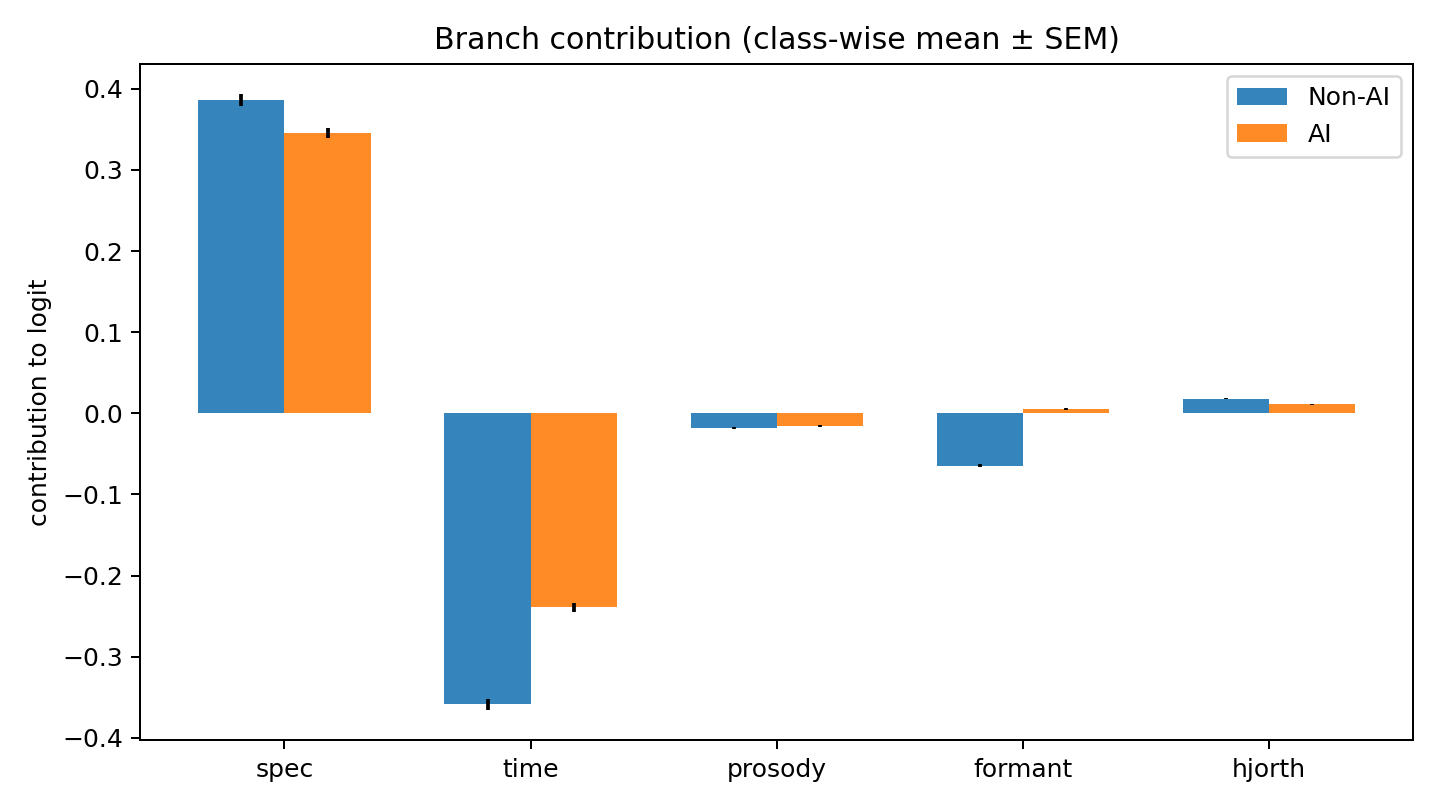
\includegraphics[width=0.7\linewidth]{images_in_paper/contrib_means_by_class.png}
  \caption{各分支在 AI 与非 AI 样本上的平均贡献值(均值±标准误差)。}
  \label{fig:contrib_means}
\end{figure}
\end{frame}
\end{document}
